% Options for packages loaded elsewhere
\PassOptionsToPackage{unicode}{hyperref}
\PassOptionsToPackage{hyphens}{url}
%
\documentclass[
]{book}
\usepackage{amsmath,amssymb}
\usepackage{iftex}
\ifPDFTeX
  \usepackage[T1]{fontenc}
  \usepackage[utf8]{inputenc}
  \usepackage{textcomp} % provide euro and other symbols
\else % if luatex or xetex
  \usepackage{unicode-math} % this also loads fontspec
  \defaultfontfeatures{Scale=MatchLowercase}
  \defaultfontfeatures[\rmfamily]{Ligatures=TeX,Scale=1}
\fi
\usepackage{lmodern}
\ifPDFTeX\else
  % xetex/luatex font selection
\fi
% Use upquote if available, for straight quotes in verbatim environments
\IfFileExists{upquote.sty}{\usepackage{upquote}}{}
\IfFileExists{microtype.sty}{% use microtype if available
  \usepackage[]{microtype}
  \UseMicrotypeSet[protrusion]{basicmath} % disable protrusion for tt fonts
}{}
\makeatletter
\@ifundefined{KOMAClassName}{% if non-KOMA class
  \IfFileExists{parskip.sty}{%
    \usepackage{parskip}
  }{% else
    \setlength{\parindent}{0pt}
    \setlength{\parskip}{6pt plus 2pt minus 1pt}}
}{% if KOMA class
  \KOMAoptions{parskip=half}}
\makeatother
\usepackage{xcolor}
\usepackage{color}
\usepackage{fancyvrb}
\newcommand{\VerbBar}{|}
\newcommand{\VERB}{\Verb[commandchars=\\\{\}]}
\DefineVerbatimEnvironment{Highlighting}{Verbatim}{commandchars=\\\{\}}
% Add ',fontsize=\small' for more characters per line
\usepackage{framed}
\definecolor{shadecolor}{RGB}{248,248,248}
\newenvironment{Shaded}{\begin{snugshade}}{\end{snugshade}}
\newcommand{\AlertTok}[1]{\textcolor[rgb]{0.94,0.16,0.16}{#1}}
\newcommand{\AnnotationTok}[1]{\textcolor[rgb]{0.56,0.35,0.01}{\textbf{\textit{#1}}}}
\newcommand{\AttributeTok}[1]{\textcolor[rgb]{0.13,0.29,0.53}{#1}}
\newcommand{\BaseNTok}[1]{\textcolor[rgb]{0.00,0.00,0.81}{#1}}
\newcommand{\BuiltInTok}[1]{#1}
\newcommand{\CharTok}[1]{\textcolor[rgb]{0.31,0.60,0.02}{#1}}
\newcommand{\CommentTok}[1]{\textcolor[rgb]{0.56,0.35,0.01}{\textit{#1}}}
\newcommand{\CommentVarTok}[1]{\textcolor[rgb]{0.56,0.35,0.01}{\textbf{\textit{#1}}}}
\newcommand{\ConstantTok}[1]{\textcolor[rgb]{0.56,0.35,0.01}{#1}}
\newcommand{\ControlFlowTok}[1]{\textcolor[rgb]{0.13,0.29,0.53}{\textbf{#1}}}
\newcommand{\DataTypeTok}[1]{\textcolor[rgb]{0.13,0.29,0.53}{#1}}
\newcommand{\DecValTok}[1]{\textcolor[rgb]{0.00,0.00,0.81}{#1}}
\newcommand{\DocumentationTok}[1]{\textcolor[rgb]{0.56,0.35,0.01}{\textbf{\textit{#1}}}}
\newcommand{\ErrorTok}[1]{\textcolor[rgb]{0.64,0.00,0.00}{\textbf{#1}}}
\newcommand{\ExtensionTok}[1]{#1}
\newcommand{\FloatTok}[1]{\textcolor[rgb]{0.00,0.00,0.81}{#1}}
\newcommand{\FunctionTok}[1]{\textcolor[rgb]{0.13,0.29,0.53}{\textbf{#1}}}
\newcommand{\ImportTok}[1]{#1}
\newcommand{\InformationTok}[1]{\textcolor[rgb]{0.56,0.35,0.01}{\textbf{\textit{#1}}}}
\newcommand{\KeywordTok}[1]{\textcolor[rgb]{0.13,0.29,0.53}{\textbf{#1}}}
\newcommand{\NormalTok}[1]{#1}
\newcommand{\OperatorTok}[1]{\textcolor[rgb]{0.81,0.36,0.00}{\textbf{#1}}}
\newcommand{\OtherTok}[1]{\textcolor[rgb]{0.56,0.35,0.01}{#1}}
\newcommand{\PreprocessorTok}[1]{\textcolor[rgb]{0.56,0.35,0.01}{\textit{#1}}}
\newcommand{\RegionMarkerTok}[1]{#1}
\newcommand{\SpecialCharTok}[1]{\textcolor[rgb]{0.81,0.36,0.00}{\textbf{#1}}}
\newcommand{\SpecialStringTok}[1]{\textcolor[rgb]{0.31,0.60,0.02}{#1}}
\newcommand{\StringTok}[1]{\textcolor[rgb]{0.31,0.60,0.02}{#1}}
\newcommand{\VariableTok}[1]{\textcolor[rgb]{0.00,0.00,0.00}{#1}}
\newcommand{\VerbatimStringTok}[1]{\textcolor[rgb]{0.31,0.60,0.02}{#1}}
\newcommand{\WarningTok}[1]{\textcolor[rgb]{0.56,0.35,0.01}{\textbf{\textit{#1}}}}
\usepackage{longtable,booktabs,array}
\usepackage{calc} % for calculating minipage widths
% Correct order of tables after \paragraph or \subparagraph
\usepackage{etoolbox}
\makeatletter
\patchcmd\longtable{\par}{\if@noskipsec\mbox{}\fi\par}{}{}
\makeatother
% Allow footnotes in longtable head/foot
\IfFileExists{footnotehyper.sty}{\usepackage{footnotehyper}}{\usepackage{footnote}}
\makesavenoteenv{longtable}
\usepackage{graphicx}
\makeatletter
\def\maxwidth{\ifdim\Gin@nat@width>\linewidth\linewidth\else\Gin@nat@width\fi}
\def\maxheight{\ifdim\Gin@nat@height>\textheight\textheight\else\Gin@nat@height\fi}
\makeatother
% Scale images if necessary, so that they will not overflow the page
% margins by default, and it is still possible to overwrite the defaults
% using explicit options in \includegraphics[width, height, ...]{}
\setkeys{Gin}{width=\maxwidth,height=\maxheight,keepaspectratio}
% Set default figure placement to htbp
\makeatletter
\def\fps@figure{htbp}
\makeatother
\setlength{\emergencystretch}{3em} % prevent overfull lines
\providecommand{\tightlist}{%
  \setlength{\itemsep}{0pt}\setlength{\parskip}{0pt}}
\setcounter{secnumdepth}{5}
\usepackage{booktabs}
\usepackage{longtable}
\usepackage[bf,singlelinecheck=off]{caption}
\usepackage{graphicx}
\usepackage{Alegreya}
\usepackage[scale=.7]{sourcecodepro}

\usepackage{framed,color}
\definecolor{shadecolor}{RGB}{248,248,248}

\renewcommand{\textfraction}{0.05}
\renewcommand{\topfraction}{0.8}
\renewcommand{\bottomfraction}{0.8}
\renewcommand{\floatpagefraction}{0.75}

\renewenvironment{quote}{\begin{VF}}{\end{VF}}
\let\oldhref\href
\renewcommand{\href}[2]{#2\footnote{\url{#1}}}

\ifxetex
  \usepackage{letltxmacro}
  \setlength{\XeTeXLinkMargin}{1pt}
  \LetLtxMacro\SavedIncludeGraphics\includegraphics
  \def\includegraphics#1#{% #1 catches optional stuff (star/opt. arg.)
    \IncludeGraphicsAux{#1}%
  }%
  \newcommand*{\IncludeGraphicsAux}[2]{%
    \XeTeXLinkBox{%
      \SavedIncludeGraphics#1{#2}%
    }%
  }%
\fi

\makeatletter
\newenvironment{kframe}{%
\medskip{}
\setlength{\fboxsep}{.8em}
 \def\at@end@of@kframe{}%
 \ifinner\ifhmode%
  \def\at@end@of@kframe{\end{minipage}}%
  \begin{minipage}{\columnwidth}%
 \fi\fi%
 \def\FrameCommand##1{\hskip\@totalleftmargin \hskip-\fboxsep
 \colorbox{shadecolor}{##1}\hskip-\fboxsep
     % There is no \\@totalrightmargin, so:
     \hskip-\linewidth \hskip-\@totalleftmargin \hskip\columnwidth}%
 \MakeFramed {\advance\hsize-\width
   \@totalleftmargin\z@ \linewidth\hsize
   \@setminipage}}%
 {\par\unskip\endMakeFramed%
 \at@end@of@kframe}
\makeatother

\makeatletter
\@ifundefined{Shaded}{
}{\renewenvironment{Shaded}{\begin{kframe}}{\end{kframe}}}
\makeatother

\newenvironment{rmdblock}[1]
  {
  \begin{itemize}
  \renewcommand{\labelitemi}{
    \raisebox{-.7\height}[0pt][0pt]{
      {\setkeys{Gin}{width=3em,keepaspectratio}\includegraphics{images/#1}}
    }
  }
  \setlength{\fboxsep}{1em}
  \begin{kframe}
  \item
  }
  {
  \end{kframe}
  \end{itemize}
  }
\newenvironment{rmdnote}
  {\begin{rmdblock}{note}}
  {\end{rmdblock}}
\newenvironment{rmdcaution}
  {\begin{rmdblock}{caution}}
  {\end{rmdblock}}
\newenvironment{rmdimportant}
  {\begin{rmdblock}{important}}
  {\end{rmdblock}}
\newenvironment{rmdtip}
  {\begin{rmdblock}{tip}}
  {\end{rmdblock}}
\newenvironment{rmdwarning}
  {\begin{rmdblock}{warning}}
  {\end{rmdblock}}

\usepackage{makeidx}
\makeindex

\urlstyle{tt}

\usepackage{amsthm}
\makeatletter
\def\thm@space@setup{%
  \thm@preskip=8pt plus 2pt minus 4pt
  \thm@postskip=\thm@preskip
}
\makeatother

\frontmatter
\ifLuaTeX
  \usepackage{selnolig}  % disable illegal ligatures
\fi
\usepackage[]{natbib}
\bibliographystyle{plainnat}
\IfFileExists{bookmark.sty}{\usepackage{bookmark}}{\usepackage{hyperref}}
\IfFileExists{xurl.sty}{\usepackage{xurl}}{} % add URL line breaks if available
\urlstyle{same}
\hypersetup{
  pdftitle={Phân tích Chuỗi thời gian},
  pdfauthor={Lê Huỳnh Đức},
  hidelinks,
  pdfcreator={LaTeX via pandoc}}

\title{Phân tích Chuỗi thời gian}
\author{Lê Huỳnh Đức}
\date{2023-12-26}

\begin{document}
\maketitle

%\cleardoublepage\newpage\thispagestyle{empty}\null
%\cleardoublepage\newpage\thispagestyle{empty}\null
%\cleardoublepage\newpage
\thispagestyle{empty}
\begin{center}

\includegraphics{images/dedication.pdf}
\end{center}

\setlength{\abovedisplayskip}{-5pt}
\setlength{\abovedisplayshortskip}{-5pt}

{
\setcounter{tocdepth}{2}
\tableofcontents
}
\hypertarget{lux1eddi-nuxf3i-ux111ux1ea7u}{%
\chapter*{Lời nói đầu}\label{lux1eddi-nuxf3i-ux111ux1ea7u}}


\hypertarget{giux1edbi-thiux1ec7u-cux1a1-bux1ea3n-vux1ec1-time-series}{%
\chapter{Giới thiệu Cơ bản về Time Series}\label{giux1edbi-thiux1ec7u-cux1a1-bux1ea3n-vux1ec1-time-series}}

\hypertarget{time-series-luxe0-guxec}{%
\section{Time Series là gì}\label{time-series-luxe0-guxec}}

Chuỗi thời gian là tập hợp các quan sát \(y_t\) theo thời gian tuần tự.

Chuỗi thời gian rời rạc là tập hợp các điểm quan sát có khoảng cách quan sát lớn hơn một giây. Chuỗi thời gian rời rạc có thể có những đặc điểm:

\begin{itemize}
\item
  Thời gian thu thập các điểm dữ liệu có thể là không thường xuyên ( mỗi điểm mỗi phút) hoặc không quy tắc (hành vi đăng nhập của người dùng tại bất cứ thời điểm nào).
\item
  Có thể bị mất dữ liệu do mất kết nối mạng hoặc máy chủ không phản hồi.
\end{itemize}

Chuỗi thời gian liên tục là tập hợp các điểm quan sát có khoảng cách quan sát là một giây.

\textbf{Thời gian là gì}

Thời gian có thể định nghĩa theo:

\begin{itemize}
\tightlist
\item
  Giờ, phút giây
\item
  Theo không gian: Máy thứ nhất, máy thứ hai trong cùng một băng chuyền
\item
  Theo độ sâu: Xuống 1 milimet, xuống 2 milimet
\end{itemize}

Tóm lại, miễn các thông tin tuân theo thời gian và có hướng giá trị tuân theo

\begin{center}\rule{0.5\linewidth}{0.5pt}\end{center}

\hypertarget{cuxe1c-patterns-time-series}{%
\section{Các patterns Time Series}\label{cuxe1c-patterns-time-series}}

Khi mô tả về chuỗi thời gian, chúng ta thường nhắc đến các yếu tố như xu hướng, chu kỳ và theo mùa.

\textbf{\emph{Xu hướng}}

Chúng ta nói dữ liệu có tính xu hướng khi nó tăng hoặc giảm trong một thời gian dài, xu hướng không nhất thiết phải là tăng/giảm tuyến tính, nó có thể là đường cong. Một chuỗi thời gian có thể tồn tại cả xu hướng tăng và xu hướng giảm cùng một lúc.

Ví dụ về dân số Việt Nam có xu hướng tăng hằng năm
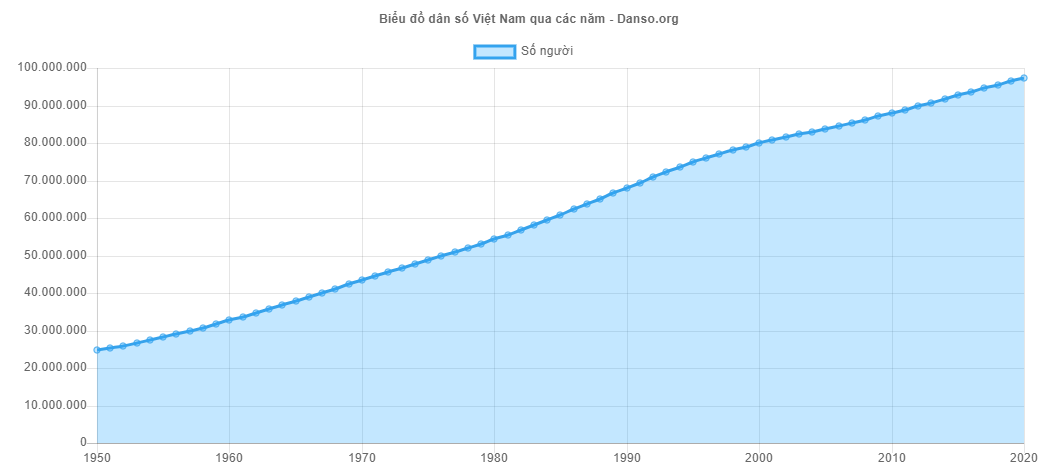
\includegraphics{../images/01/danso.png}

Ví dụ về tỉ lệ tử vong của trẻ sơ sinh có xu hướng giảm dần thời gian nhờ có sự tiến bộ về y tế
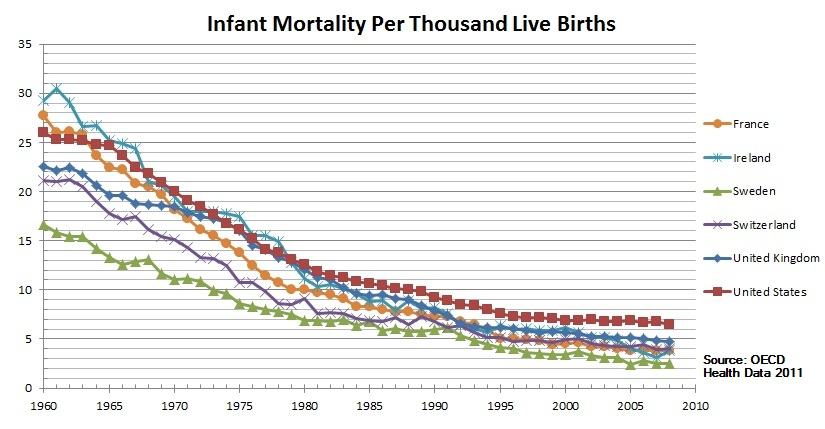
\includegraphics{https://upload.wikimedia.org/wikipedia/commons/1/15/First-World-Infant-Mortality-Trends.jpg}

Ví dụ về sự thay đổi của giá Bitcoin theo thời gian, giá bitcoin có xu hướng tăng mạnh từ giữa tháng 08/2020 đến 03/2021, đến tháng 11/2021 bắt đầu có xu hướng giảm dần
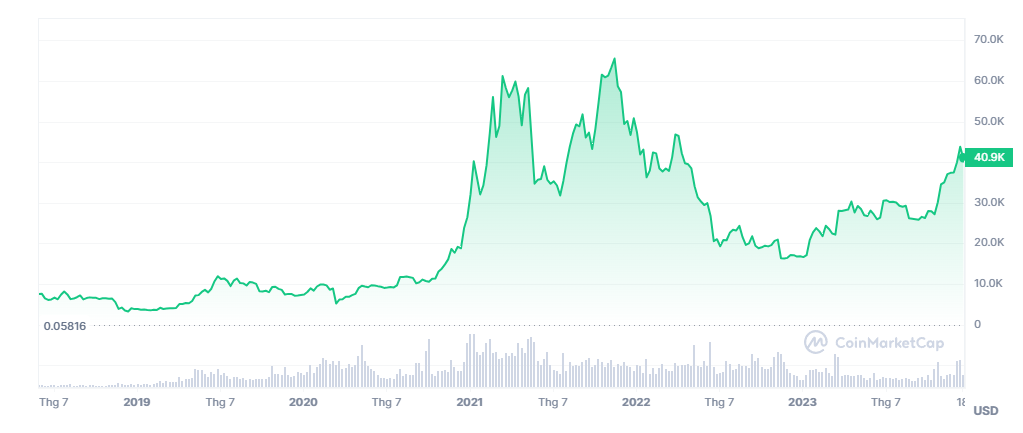
\includegraphics{../images/01/coin.png}

\textbf{\emph{Thời vụ}}

Một chuỗi thời gian có tính chất thời vụ khi các giá trị của chuỗi thời gian bị ảnh hưởng bởi thời điểm nào đó trong năm hoặc theo ngày của mỗi tuần. Tính chất thời vụ luôn có tần suất tăng/giảm cố định và đã biết trước.
Ví dụ như

\begin{itemize}
\item
  Số lượng hành khách đặt vé máy bay tăng cao vào các ngày lễ tết.
\item
  Lượng khách trong nhà hàng tăng cao vào các ngày cuối tuần.
\item
  Lượng quần áo mua cao nhất vào tháng 12 cuối năm và thấp nhất vào tháng 1 mỗi năm
\end{itemize}

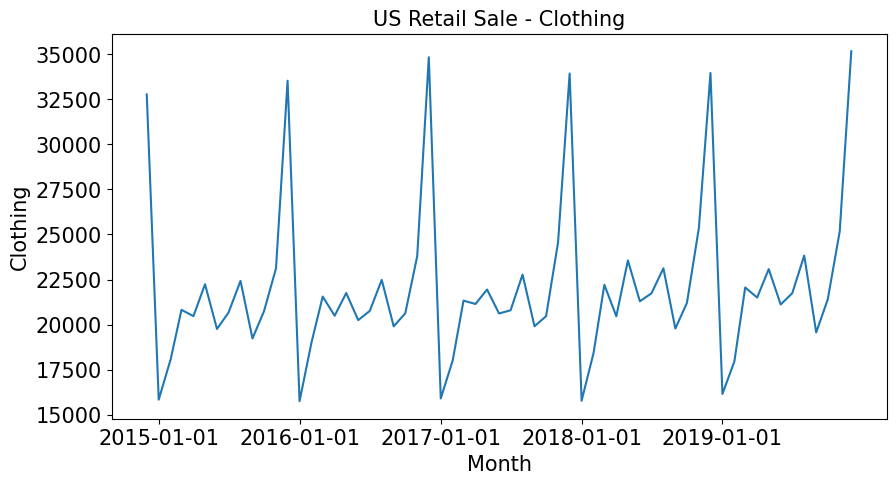
\includegraphics{../images/01/seasonal.png}

\textbf{\emph{Chu kì}}

Biến đổi chu kỳ xảy ra khi một dữ liệu tăng giảm không có tần suất cố định. Những biến động này thường xảy ra do điều kiện kinh tế và hay gọi là ``chu kì kinh doanh''. Độ dài của một chu kì thường ít nhất là 2 năm.

\includegraphics{https://sciencetheory.net/wp-content/uploads/2020/03/Business-Cycle-Graph-e1577193470836.png}

\textbf{\emph{Irregularity}}
Unexpected situations/events/scenarios and spikes in a short time span.

\begin{center}\rule{0.5\linewidth}{0.5pt}\end{center}

\hypertarget{cuxe1c-ux111ux1eb7c-ux111iux1ec3m-cux1ee7a-time-series}{%
\section{Các đặc điểm của Time Series}\label{cuxe1c-ux111ux1eb7c-ux111iux1ec3m-cux1ee7a-time-series}}

\hypertarget{stationary-tuxednh-dux1eebng-cux1ee7a-dux1eef-liux1ec7u}{%
\subsection{Stationary (Tính dừng của dữ liệu)}\label{stationary-tuxednh-dux1eebng-cux1ee7a-dux1eef-liux1ec7u}}

Chuỗi thời gian dừng là chuỗi có các đặc trưng thống kê như mean, variance, autocorrelation không đổi theo thời gian.

\hypertarget{lag}{%
\subsection{Lag}\label{lag}}

Lag của Time Series thể hiện việc lùi về một mốc trước đó. Ví dụ lag(1) nghĩa là lùi về trước đó 1 đơn vị \(X_{T-1}\). Lag(n) nghĩa là lùi về trước đó n đơn vị \(X_{T-n}\)

Ví dụ về số lượng quần áo bán ra của US từ năm 1992 đến năm 2019

\begin{Shaded}
\begin{Highlighting}[]
\NormalTok{df }\OperatorTok{=}\NormalTok{ pd.read\_csv(}\StringTok{\textquotesingle{}../data/us{-}retail{-}sales.csv\textquotesingle{}}\NormalTok{)}
\NormalTok{df}
\end{Highlighting}
\end{Shaded}

\begin{verbatim}
         Month  Clothing
0   1992-01-01  6938
1   1992-02-01  7524
2   1992-03-01  8475
3   1992-04-01  9401
4   1992-05-01  9558
... ... ...
331 2019-08-01  23829
332 2019-09-01  19567
333 2019-10-01  21400
334 2019-11-01  25170
335 2019-12-01  35157
\end{verbatim}

Trong pandas, để tìm lag, ta dùng phương thức \texttt{shift}. Ví dụ

\begin{Shaded}
\begin{Highlighting}[]
\NormalTok{df[}\StringTok{\textquotesingle{}lag\_1\textquotesingle{}}\NormalTok{] }\OperatorTok{=}\NormalTok{ df[}\StringTok{\textquotesingle{}Clothing\textquotesingle{}}\NormalTok{].shift(}\DecValTok{1}\NormalTok{)}
\NormalTok{df[}\StringTok{\textquotesingle{}lag\_3\textquotesingle{}}\NormalTok{] }\OperatorTok{=}\NormalTok{ df[}\StringTok{\textquotesingle{}Clothing\textquotesingle{}}\NormalTok{].shift(}\DecValTok{3}\NormalTok{)}
\NormalTok{df[}\StringTok{\textquotesingle{}lag\_12\textquotesingle{}}\NormalTok{] }\OperatorTok{=}\NormalTok{ df[}\StringTok{\textquotesingle{}Clothing\textquotesingle{}}\NormalTok{].shift(}\DecValTok{12}\NormalTok{)}
\NormalTok{df}
\end{Highlighting}
\end{Shaded}

\begin{verbatim}
         Month  Clothing    lag_1    lag_3   lag_12
0   1992-01-01      6938      NaN      NaN      NaN
1   1992-02-01      7524   6938.0      NaN      NaN
2   1992-03-01      8475   7524.0      NaN      NaN
3   1992-04-01      9401   8475.0   6938.0      NaN
4   1992-05-01      9558   9401.0   7524.0      NaN
..         ...       ...      ...      ...      ...
331 2019-08-01     23829  21742.0  23079.0  23121.0
332 2019-09-01     19567  23829.0  21116.0  19782.0
333 2019-10-01     21400  19567.0  21742.0  21203.0
334 2019-11-01     25170  21400.0  23829.0  25364.0
335 2019-12-01     35157  25170.0  19567.0  33950.0
\end{verbatim}

\hypertarget{autocorrelation-tux1ef1-tux1b0ux1a1ng-quan}{%
\subsection{Autocorrelation (Tự tương quan)}\label{autocorrelation-tux1ef1-tux1b0ux1a1ng-quan}}

\textbf{Correlation}

Correlation là tương quan giữa 2 biến khác nhau, giá trị correlation nằm trong khoảng từ -1 đến 1, nếu giá trị càng tiến -1 nghĩa là 2 biến có sự tương quan nghịch, giá trị càng tiến đến +1 nghĩa là 2 biến có sự tương quan thuận

\textbf{Autocorrelation}

Autocorrelation là tương quan giữa một chuỗi timeseries và chuỗi đó với giá trị trước đó của chính nó.
Ví dụ tương quan giữa \texttt{Clothing} và \texttt{lag\_1}

\begin{Shaded}
\begin{Highlighting}[]
\NormalTok{df[[}\StringTok{\textquotesingle{}Clothing\textquotesingle{}}\NormalTok{,}\StringTok{\textquotesingle{}lag\_1\textquotesingle{}}\NormalTok{]].corr()}
\end{Highlighting}
\end{Shaded}

\begin{Shaded}
\begin{Highlighting}[]
\NormalTok{            Clothing       lag\_1}
\NormalTok{Clothing    }\FloatTok{1.000000}    \FloatTok{0.518296}
\NormalTok{lag\_1       }\FloatTok{0.518296}    \FloatTok{1.000000}
\end{Highlighting}
\end{Shaded}

Tương quan giữa 2 biến này là 0.5

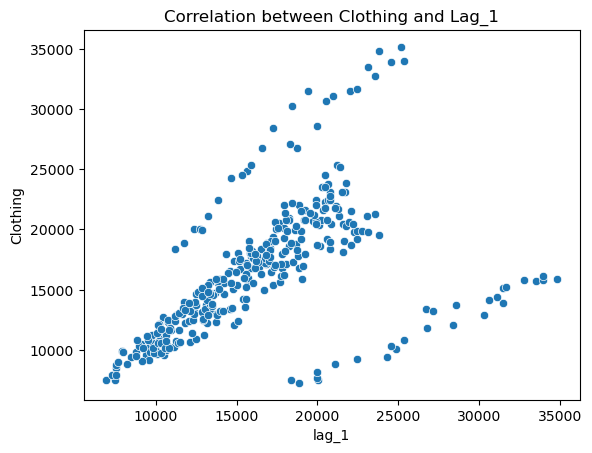
\includegraphics{../images/01/lag_corr.png}

Để tính correlation giữa Timeseries và các lag của nó, ta sử dụng hàm \texttt{acf} trong statsmodel

\begin{Shaded}
\begin{Highlighting}[]
\ImportTok{from}\NormalTok{ statsmodels.api }\ImportTok{import}\NormalTok{ tsa}
\NormalTok{tsa.acf(df[}\StringTok{\textquotesingle{}Clothing\textquotesingle{}}\NormalTok{])}
\end{Highlighting}
\end{Shaded}

\begin{Shaded}
\begin{Highlighting}[]
\NormalTok{array([}\FloatTok{1.}\NormalTok{        , }\FloatTok{0.50679045}\NormalTok{, }\FloatTok{0.42793583}\NormalTok{, }\FloatTok{0.48943282}\NormalTok{, }\FloatTok{0.54920848}\NormalTok{,}
       \FloatTok{0.51760066}\NormalTok{, }\FloatTok{0.47709491}\NormalTok{, }\FloatTok{0.50840091}\NormalTok{, }\FloatTok{0.5311846}\NormalTok{ , }\FloatTok{0.46104267}\NormalTok{,}
       \FloatTok{0.38738473}\NormalTok{, }\FloatTok{0.45582436}\NormalTok{, }\FloatTok{0.9264336}\NormalTok{ , }\FloatTok{0.45220705}\NormalTok{, }\FloatTok{0.37936738}\NormalTok{,}
       \FloatTok{0.43736208}\NormalTok{, }\FloatTok{0.49102051}\NormalTok{, }\FloatTok{0.46205604}\NormalTok{, }\FloatTok{0.42158496}\NormalTok{, }\FloatTok{0.4519868}\NormalTok{ ,}
       \FloatTok{0.47432784}\NormalTok{, }\FloatTok{0.403097}\NormalTok{  , }\FloatTok{0.33531148}\NormalTok{, }\FloatTok{0.40104508}\NormalTok{, }\FloatTok{0.85039363}\NormalTok{,}
       \FloatTok{0.39243258}\NormalTok{])}
\end{Highlighting}
\end{Shaded}

Ở đây correlation giữa \texttt{Clothing} và \texttt{lag\_1} là 0.507, hơi khác so với dùng pandas, trong khuôn khổ phần này ta tập trung vào thư viện statsmodel hơn

Để visualize các giá trị correlation này ta dùng hàm \texttt{plot\_acf}, ví dụ vẽ autocorrelation với lag tối đa là 30

\begin{Shaded}
\begin{Highlighting}[]
\ImportTok{import}\NormalTok{ matplotlib.pyplot }\ImportTok{as}\NormalTok{ plt}
\ImportTok{from}\NormalTok{ statsmodels.graphics.tsaplots }\ImportTok{import}\NormalTok{ plot\_acf}
\NormalTok{fig, ax }\OperatorTok{=}\NormalTok{ plt.subplots(figsize}\OperatorTok{=}\NormalTok{(}\DecValTok{10}\NormalTok{, }\DecValTok{5}\NormalTok{))}
\NormalTok{plot\_acf(df[}\StringTok{\textquotesingle{}Clothing\textquotesingle{}}\NormalTok{], lags}\OperatorTok{=}\DecValTok{30}\NormalTok{, ax}\OperatorTok{=}\NormalTok{ax)}
\NormalTok{\_ }\OperatorTok{=}\NormalTok{plt.xticks(}\BuiltInTok{list}\NormalTok{(}\BuiltInTok{range}\NormalTok{(}\DecValTok{31}\NormalTok{)))}
\NormalTok{plt.show()}
\end{Highlighting}
\end{Shaded}

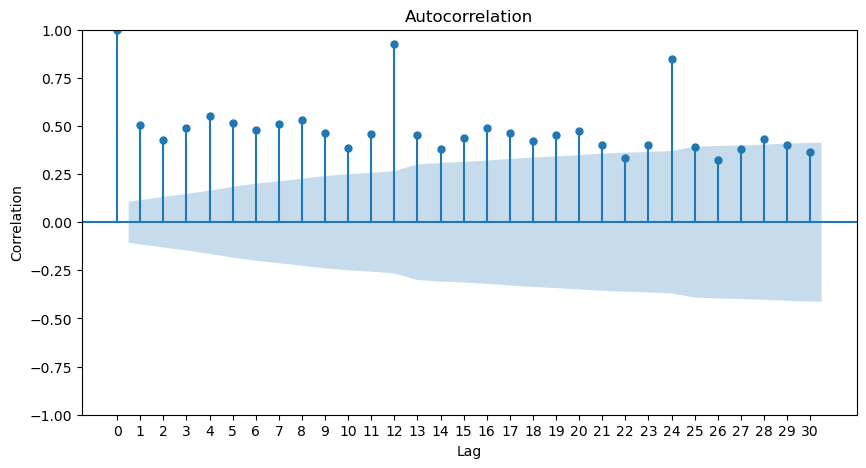
\includegraphics{../images/01/auto_corr.png}

Trong hình vẽ ta có thể thấy, correlation tại lag=12 và lag=24 có giá trị rất cao, do đó có thể suy đoán được timeseries này có tính tuần hoàn sau 12 tháng

\hypertarget{ux1ee9ng-dux1ee5ng-cux1ee7a-autocorrelation}{%
\subsubsection{Ứng dụng của Autocorrelation}\label{ux1ee9ng-dux1ee5ng-cux1ee7a-autocorrelation}}

\begin{itemize}
\tightlist
\item
  \textbf{Xử lý Tín Hiệu và Thời Gian}:

  \begin{itemize}
  \tightlist
  \item
    \textbf{Phân tích chuỗi thời gian}: Được sử dụng để phát hiện chu kỳ, mô hình chuỗi thời gian, và dự đoán giá trị trong tương lai.
  \item
    \textbf{Xử lý âm thanh}: Trong xử lý tín hiệu âm thanh, tự động tương quan có thể được sử dụng để phát hiện các tần số quan trọng và các sự kiện lặp lại trong dữ liệu âm thanh.
  \end{itemize}
\item
  \textbf{Khoa học Dữ Liệu}:

  \begin{itemize}
  \tightlist
  \item
    \textbf{Phân tích dữ liệu}: Trong khoa học dữ liệu và thống kê, tự động tương quan giúp phát hiện mối tương quan giữa các biến và mô tả sự phụ thuộc thời gian của dữ liệu.
  \item
    \textbf{Phát hiện xu hướng và chu kỳ}: Tự động tương quan có thể giúp xác định xu hướng và chu kỳ trong dữ liệu, giúp các nhà nghiên cứu và chuyên gia dự đoán và phân tích xu hướng thị trường, tình hình thời tiết, và nhiều ứng dụng khác.
  \end{itemize}
\item
  \textbf{Kỹ thuật và Kỹ thuật số}:

  \begin{itemize}
  \tightlist
  \item
    \textbf{Xử lý ảnh}: Trong xử lý ảnh, tự động tương quan có thể được sử dụng để phát hiện biến đổi không gian và mô hình hình dạng.
  \item
    \textbf{Kỹ thuật số và mạng truyền thông}: Trong mạng truyền thông số và kỹ thuật số, tự động tương quan giúp phân tích tín hiệu, phát hiện tín hiệu trong nhiễu và cải thiện chất lượng truyền thông.
  \end{itemize}
\item
  \textbf{Tài chính và Kinh tế}:

  \begin{itemize}
  \tightlist
  \item
    Phân tích thị trường: Trong tài chính, tự động tương quan giúp phân tích và dự đoán xu hướng thị trường, giúp các nhà giao dịch và nhà đầu tư hiểu rõ hơn về sự biến động và rủi ro trong thị trường tài chính.
  \end{itemize}
\item
  \textbf{Khoa học và Tâm lý học}:

  \begin{itemize}
  \tightlist
  \item
    \textbf{Nghiên cứu tâm lý}: Trong nghiên cứu tâm lý, tự động tương quan có thể được sử dụng để phân tích sự phụ thuộc thời gian của các biến tâm lý và hành vi, giúp hiểu rõ hơn về sự ảnh hưởng và tương tác giữa các yếu tố khác nhau trong tâm lý học.
    Như vậy, tự động tương quan là một công cụ quan trọng và linh hoạt, được sử dụng rộng rãi trong nhiều lĩnh vực để phân tích, mô hình, và hiểu rõ hơn về sự phụ thuộc và tương tác trong dữ liệu và các hệ thống phức tạp.
  \end{itemize}
\end{itemize}

\hypertarget{partial-autocorrelation}{%
\subsection{Partial Autocorrelation}\label{partial-autocorrelation}}

Partial Autocorrelation cũng tương tự như Autocorrelation. Tuy nhiên, nó mở rộng hơn bằng cách loại bỏ ảnh hưởng của các mốc thời gian trước đó.

Ví dụ tương quan Partial Autocorrelation với lag = 3 sẽ bỏ qua các giá trị trễ tại lag = 1 và lag = 2

\hypertarget{cuxe1c-buxe0i-touxe1n-vux1ec1-chuux1ed7i-thux1eddi-gian}{%
\section{Các bài toán về chuỗi thời gian}\label{cuxe1c-buxe0i-touxe1n-vux1ec1-chuux1ed7i-thux1eddi-gian}}

\hypertarget{dux1ef1-ux111ouxe1n-giuxe1-trux1ecb-tiux1ebfp-theo-dux1ef1a-truxean-cuxe1c-giuxe1-trux1ecb-trux1b0ux1edbc-ux111uxf3}{%
\subsection{Dự đoán giá trị tiếp theo dựa trên các giá trị trước đó}\label{dux1ef1-ux111ouxe1n-giuxe1-trux1ecb-tiux1ebfp-theo-dux1ef1a-truxean-cuxe1c-giuxe1-trux1ecb-trux1b0ux1edbc-ux111uxf3}}

\hypertarget{phuxe2n-loux1ea1i-chuux1ed7i-thux1eddi-gian}{%
\subsection{Phân loại chuỗi thời gian}\label{phuxe2n-loux1ea1i-chuux1ed7i-thux1eddi-gian}}

\hypertarget{phuxe2n-ux111oux1ea1n-chuux1ed7i-thux1eddi-gian}{%
\subsection{Phân đoạn chuỗi thời gian}\label{phuxe2n-ux111oux1ea1n-chuux1ed7i-thux1eddi-gian}}

\hypertarget{smoothing}{%
\chapter{Smoothing}\label{smoothing}}

Kỹ thuật làm mịn là một trong các kỹ thuật tiền xử lý dữ liệu để loại bỏ các nhiễu trong dữ liệu. Việc làm mịn dữ liệu giúp xóa bỏ mùa vụ của dữ liệu và giúp đơn giản hóa các mô hình dự đoán.

Các kỹ thuật làm mịn dữ liệu bao gồm:

\begin{itemize}
\tightlist
\item
  Làm mịn trung bình trượt (Moving Average Smoothing)
\item
  Làm mịn cấp số nhân (Exponential smoothing)
\end{itemize}

\hypertarget{moving-average-smoothing}{%
\section{Moving Average Smoothing}\label{moving-average-smoothing}}

Có 2 loại trung bình trượt : Centered MA và Trailing MA

\hypertarget{centered-moving-average}{%
\subsection{Centered Moving Average}\label{centered-moving-average}}

Với trung bình trượt với cửa sổ trượt \(k\) bằng 3 ta có:

\[\begin{align}
\Large S_{T} = \frac{y_{T+1} + y_{T} + y_{T-1}}{3}
\end{align}\]

Tổng quát hơn

\[\begin{align}
\Large S_{T} = \frac{1}{m}  \sum_{j=-m}^{m}{y_{T+j}}
\end{align}\]

Trong đó \(k = 2m + 1\)

Phương pháp này sử dụng giá trị tương lai \(y_{T+1}\) do đó không áp dụng được vào các mô hình dự báo. Phương pháp dùng để thống kê mô tả dữ liệu

\hypertarget{trailing-moving-average}{%
\subsection{Trailing Moving Average}\label{trailing-moving-average}}

Với trung bình trượt với cửa sổ trượt \(k\) bằng 3 ta có

\[\begin{align}
\Large S_{T} = \frac{y_{T} + y_{T - 1} + y_{T - 2}}{3}
\end{align}\]

Tổng quát hơn

\[\begin{align}
\Large S_{T} = \frac{1}{k} \sum^{k}_{i=1}{y_{T-i+1}}
\end{align}\]

Phương pháp này chỉ sử dụng dữ liệu quá khứ nên có thể áp dụng cho việc dự báo các giá trị tương lai

\hypertarget{vuxed-dux1ee5}{%
\subsection{Ví dụ}\label{vuxed-dux1ee5}}

Dưới đây là ví dụ về số bé gái sinh ra mỗi ngày

\begin{Shaded}
\begin{Highlighting}[]
\NormalTok{df }\OperatorTok{=}\NormalTok{ pd.read\_csv(}\StringTok{\textquotesingle{}../data/daily{-}total{-}female{-}births.csv\textquotesingle{}}\NormalTok{)}
\NormalTok{df[}\StringTok{\textquotesingle{}Date\textquotesingle{}}\NormalTok{] }\OperatorTok{=}\NormalTok{ pd.to\_datetime(df[}\StringTok{\textquotesingle{}Date\textquotesingle{}}\NormalTok{])}
\NormalTok{df[}\StringTok{\textquotesingle{}lag\_1\textquotesingle{}}\NormalTok{] }\OperatorTok{=}\NormalTok{ df[}\StringTok{\textquotesingle{}Births\textquotesingle{}}\NormalTok{].shift(}\DecValTok{1}\NormalTok{)}
\NormalTok{df[}\StringTok{\textquotesingle{}lag\_2\textquotesingle{}}\NormalTok{] }\OperatorTok{=}\NormalTok{ df[}\StringTok{\textquotesingle{}Births\textquotesingle{}}\NormalTok{].shift(}\DecValTok{2}\NormalTok{)}
\NormalTok{df[}\StringTok{\textquotesingle{}lead\_1\textquotesingle{}}\NormalTok{] }\OperatorTok{=}\NormalTok{ df[}\StringTok{\textquotesingle{}Births\textquotesingle{}}\NormalTok{].shift(}\OperatorTok{{-}}\DecValTok{1}\NormalTok{)}
\NormalTok{df[}\StringTok{\textquotesingle{}Centered\_MA\textquotesingle{}}\NormalTok{] }\OperatorTok{=}\NormalTok{ (df[}\StringTok{\textquotesingle{}Births\textquotesingle{}}\NormalTok{] }\OperatorTok{+}\NormalTok{ df[}\StringTok{\textquotesingle{}lead\_1\textquotesingle{}}\NormalTok{] }\OperatorTok{+}\NormalTok{ df[}\StringTok{\textquotesingle{}lag\_1\textquotesingle{}}\NormalTok{])}\OperatorTok{/}\DecValTok{3}
\NormalTok{df[}\StringTok{\textquotesingle{}Trailing\_MA\textquotesingle{}}\NormalTok{] }\OperatorTok{=}\NormalTok{ (df[}\StringTok{\textquotesingle{}Births\textquotesingle{}}\NormalTok{] }\OperatorTok{+}\NormalTok{ df[}\StringTok{\textquotesingle{}lag\_1\textquotesingle{}}\NormalTok{] }\OperatorTok{+}\NormalTok{ df[}\StringTok{\textquotesingle{}lag\_2\textquotesingle{}}\NormalTok{])}\OperatorTok{/}\DecValTok{3}
\end{Highlighting}
\end{Shaded}

\begin{verbatim}
          Date Births   lag_1   lag_2   lead_1  Centered_MA Trailing_MA Births_MA
0   1959-01-01     35     NaN     NaN     32.0          NaN         NaN       NaN
1   1959-01-02     32    35.0     NaN     30.0    32.333333         NaN       NaN
2   1959-01-03     30    32.0    35.0     31.0    31.000000   32.333333       NaN
3   1959-01-04     31    30.0    32.0     44.0    35.000000   31.000000       NaN
4   1959-01-05     44    31.0    30.0     29.0    34.666667   35.000000       NaN
...        ...    ...     ...     ...      ...          ...         ...       ...
360 1959-12-27     37    34.0    44.0     52.0    41.000000   38.333333 41.666667
361 1959-12-28     52    37.0    34.0     48.0    45.666667   41.000000 41.666667
362 1959-12-29     48    52.0    37.0     55.0    51.666667   45.666667 42.416667
363 1959-12-30     55    48.0    52.0     50.0    51.000000   51.666667 43.666667
364 1959-12-31     50    55.0    48.0      NaN          NaN   51.000000 44.333333
\end{verbatim}

Ta cũng có thể sử dụng phương thức \texttt{rolling()} trong Pandas

\begin{Shaded}
\begin{Highlighting}[]
\NormalTok{df[}\StringTok{\textquotesingle{}Centered\_MA\textquotesingle{}}\NormalTok{] }\OperatorTok{=}\NormalTok{ df[}\StringTok{\textquotesingle{}Births\textquotesingle{}}\NormalTok{].rolling(window}\OperatorTok{=}\DecValTok{3}\NormalTok{, center}\OperatorTok{=}\VariableTok{True}\NormalTok{).mean()}
\NormalTok{df[}\StringTok{\textquotesingle{}Trailing\_MA\textquotesingle{}}\NormalTok{] }\OperatorTok{=}\NormalTok{ df[}\StringTok{\textquotesingle{}Births\textquotesingle{}}\NormalTok{].rolling(window}\OperatorTok{=}\DecValTok{3}\NormalTok{, center}\OperatorTok{=}\VariableTok{False}\NormalTok{).mean()}
\end{Highlighting}
\end{Shaded}

Để visualize dữ liệu, ta có thể dùng \texttt{seaborn}

\begin{Shaded}
\begin{Highlighting}[]
\ImportTok{import}\NormalTok{ seaborn }\ImportTok{as}\NormalTok{ sns}
\ImportTok{import}\NormalTok{ matplotlib.pyplot }\ImportTok{as}\NormalTok{ plt }

\NormalTok{plt.figure(figsize}\OperatorTok{=}\NormalTok{(}\DecValTok{10}\NormalTok{,}\DecValTok{5}\NormalTok{))}
\NormalTok{plt.title(}\StringTok{"Births"}\NormalTok{, fontsize}\OperatorTok{=}\DecValTok{15}\NormalTok{)}
\NormalTok{sns.lineplot(x}\OperatorTok{=}\StringTok{\textquotesingle{}Date\textquotesingle{}}\NormalTok{, y}\OperatorTok{=}\StringTok{\textquotesingle{}Births\textquotesingle{}}\NormalTok{, data}\OperatorTok{=}\NormalTok{df, label}\OperatorTok{=}\StringTok{\textquotesingle{}original\textquotesingle{}}\NormalTok{)}
\CommentTok{\# sns.lineplot(x=\textquotesingle{}Month\textquotesingle{}, y=\textquotesingle{}Centered\_MA\textquotesingle{}, data=df, label=\textquotesingle{}Centered\_MA\textquotesingle{})}
\NormalTok{sns.lineplot(x}\OperatorTok{=}\StringTok{\textquotesingle{}Date\textquotesingle{}}\NormalTok{, y}\OperatorTok{=}\StringTok{\textquotesingle{}Births\textquotesingle{}}\NormalTok{, data}\OperatorTok{=}\NormalTok{df, label}\OperatorTok{=}\StringTok{\textquotesingle{}Trailing\_MA\textquotesingle{}}\NormalTok{)}
\NormalTok{plt.xlabel(}\StringTok{\textquotesingle{}Date\textquotesingle{}}\NormalTok{,fontsize}\OperatorTok{=}\DecValTok{15}\NormalTok{)}
\NormalTok{plt.yticks(fontsize}\OperatorTok{=}\DecValTok{15}\NormalTok{)}
\NormalTok{plt.ylabel(}\StringTok{\textquotesingle{}Births\textquotesingle{}}\NormalTok{,fontsize}\OperatorTok{=}\DecValTok{15}\NormalTok{)}
\NormalTok{plt.legend(fontsize}\OperatorTok{=}\DecValTok{15}\NormalTok{)}
\end{Highlighting}
\end{Shaded}

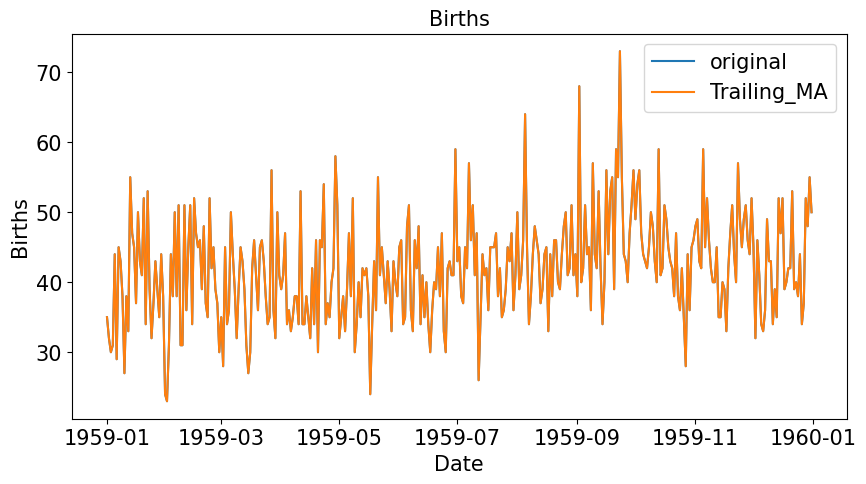
\includegraphics{../images/02/MA.png}

với các tham số \(k =6\) và \(k=12\)

\begin{Shaded}
\begin{Highlighting}[]
\NormalTok{fig1 }\OperatorTok{=}\NormalTok{ plt.figure(figsize}\OperatorTok{=}\NormalTok{(}\DecValTok{10}\NormalTok{,}\DecValTok{5}\NormalTok{))}
\NormalTok{df[}\StringTok{\textquotesingle{}Births\_MA\textquotesingle{}}\NormalTok{] }\OperatorTok{=}\NormalTok{ df[}\StringTok{\textquotesingle{}Births\textquotesingle{}}\NormalTok{].rolling(window}\OperatorTok{=}\DecValTok{6}\NormalTok{, center}\OperatorTok{=}\VariableTok{False}\NormalTok{).mean()}
\NormalTok{sns.lineplot(x}\OperatorTok{=}\StringTok{\textquotesingle{}Date\textquotesingle{}}\NormalTok{, y}\OperatorTok{=}\StringTok{\textquotesingle{}Births\textquotesingle{}}\NormalTok{, data}\OperatorTok{=}\NormalTok{df, label}\OperatorTok{=}\StringTok{\textquotesingle{}original\textquotesingle{}}\NormalTok{)}
\NormalTok{sns.lineplot(x}\OperatorTok{=}\StringTok{\textquotesingle{}Date\textquotesingle{}}\NormalTok{, y}\OperatorTok{=}\StringTok{\textquotesingle{}Births\_MA\textquotesingle{}}\NormalTok{, data}\OperatorTok{=}\NormalTok{df, label}\OperatorTok{=}\StringTok{\textquotesingle{}6{-}MA\textquotesingle{}}\NormalTok{)}
\NormalTok{plt.xlabel(}\StringTok{\textquotesingle{}Month\textquotesingle{}}\NormalTok{,fontsize}\OperatorTok{=}\DecValTok{15}\NormalTok{)}
\NormalTok{plt.xticks(fontsize}\OperatorTok{=}\DecValTok{15}\NormalTok{)}
\NormalTok{plt.yticks(fontsize}\OperatorTok{=}\DecValTok{15}\NormalTok{)}
\NormalTok{plt.ylabel(}\StringTok{\textquotesingle{}Birds\textquotesingle{}}\NormalTok{,fontsize}\OperatorTok{=}\DecValTok{15}\NormalTok{)}
\NormalTok{plt.legend(fontsize}\OperatorTok{=}\DecValTok{15}\NormalTok{)}
\NormalTok{plt.title(}\StringTok{\textquotesingle{}6{-}MA\textquotesingle{}}\NormalTok{, fontsize}\OperatorTok{=}\DecValTok{15}\NormalTok{)}
\end{Highlighting}
\end{Shaded}

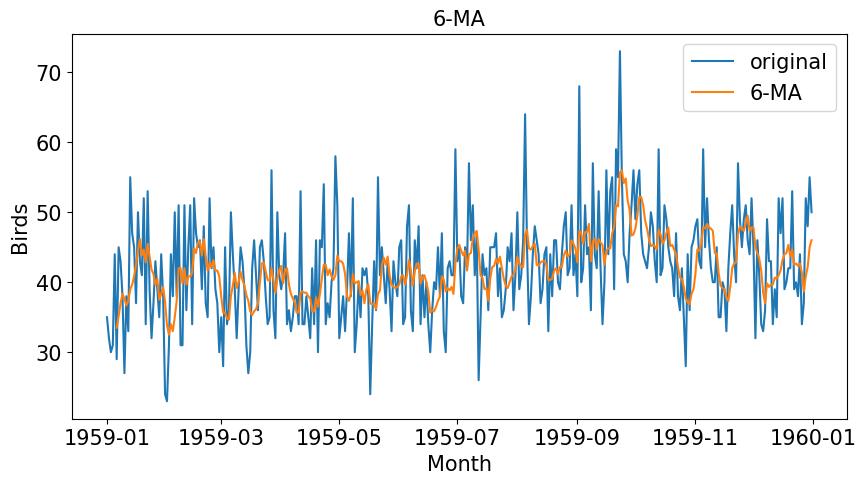
\includegraphics{../images/02/6-MA.png}

\begin{Shaded}
\begin{Highlighting}[]
\NormalTok{fig2 }\OperatorTok{=}\NormalTok{ plt.figure(figsize}\OperatorTok{=}\NormalTok{(}\DecValTok{10}\NormalTok{,}\DecValTok{5}\NormalTok{))}
\NormalTok{df[}\StringTok{\textquotesingle{}Births\_MA\textquotesingle{}}\NormalTok{] }\OperatorTok{=}\NormalTok{ df[}\StringTok{\textquotesingle{}Births\textquotesingle{}}\NormalTok{].rolling(window}\OperatorTok{=}\DecValTok{12}\NormalTok{, center}\OperatorTok{=}\VariableTok{False}\NormalTok{).mean()}
\NormalTok{sns.lineplot(x}\OperatorTok{=}\StringTok{\textquotesingle{}Date\textquotesingle{}}\NormalTok{, y}\OperatorTok{=}\StringTok{\textquotesingle{}Births\textquotesingle{}}\NormalTok{, data}\OperatorTok{=}\NormalTok{df, label}\OperatorTok{=}\StringTok{\textquotesingle{}original\textquotesingle{}}\NormalTok{)}
\NormalTok{sns.lineplot(x}\OperatorTok{=}\StringTok{\textquotesingle{}Date\textquotesingle{}}\NormalTok{, y}\OperatorTok{=}\StringTok{\textquotesingle{}Births\_MA\textquotesingle{}}\NormalTok{, data}\OperatorTok{=}\NormalTok{df, label}\OperatorTok{=}\StringTok{\textquotesingle{}12{-}MA\textquotesingle{}}\NormalTok{)}
\NormalTok{plt.xlabel(}\StringTok{\textquotesingle{}Date\textquotesingle{}}\NormalTok{,fontsize}\OperatorTok{=}\DecValTok{15}\NormalTok{)}
\NormalTok{plt.xticks(fontsize}\OperatorTok{=}\DecValTok{15}\NormalTok{)}
\NormalTok{plt.yticks(fontsize}\OperatorTok{=}\DecValTok{15}\NormalTok{)}
\NormalTok{plt.ylabel(}\StringTok{\textquotesingle{}Date\textquotesingle{}}\NormalTok{,fontsize}\OperatorTok{=}\DecValTok{15}\NormalTok{)}
\NormalTok{plt.legend(fontsize}\OperatorTok{=}\DecValTok{15}\NormalTok{)}
\NormalTok{plt.title(}\StringTok{\textquotesingle{}12{-}MA\textquotesingle{}}\NormalTok{, fontsize}\OperatorTok{=}\DecValTok{15}\NormalTok{)}
\end{Highlighting}
\end{Shaded}

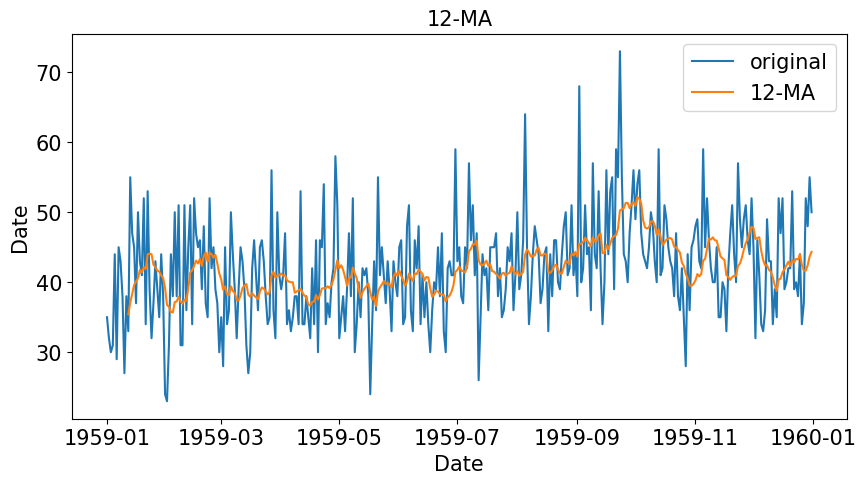
\includegraphics{../images/02/12-MA.png}

\hypertarget{exponential-smoothing}{%
\section{Exponential Smoothing}\label{exponential-smoothing}}

Hàm làm mịn Exponential là một hàm làm mịn sử dụng hàm mũ. Trong khi các hàm Moving Average đơn giản sử dụng các giá trị quá khứ với trọng số bằng nhau thì hàm Exponential sử dụng hàm số mũ cho trọng số đảm bảo giảm dần theo thời gian.

\hypertarget{simple-exponential-smoothing}{%
\subsection{Simple Exponential Smoothing}\label{simple-exponential-smoothing}}

Hàm làm mịn Exponential thường áp dụng vào xử lý tín hiệu số để lọc những nhiễu có tầm số cao. Hàm này là dạy truy hồi với công thức như sau

\(S_{0} = Y_{0}\)

\(S_{T} = \alpha Y_{T} + (1 - \alpha)S_{T-1}, T > 0\)

Trong đó \(\alpha\) được gọi là tham số smoothing và \(0 < \alpha < 1\)

\textbf{Tại sao lại gọi là Hàm mũ}

Với công thức Truy hồi trên ta có thể biến đổi như sau

\(S_T = \alpha Y_T + (1 - \alpha)S_{T-1}\)

\(S_T = \alpha Y_T + (1 - \alpha)(\alpha Y_{T-1} + (1 - \alpha)S_{T-2})\)

\(S_T = \alpha Y_T + \alpha(1 - \alpha)Y_{T-1} + (1-\alpha)^2S_{T-2}\)

\(S_T = \alpha[Y_T + (1 - \alpha)Y_{T-1} + (1-\alpha)^2Y_{T-2} + (1-\alpha)^3Y_{T-3} + ... +(1-\alpha)^TY_0]\)

Ta có thể thấy \(S_T\) có liên quan đến trung bình các giá trị với các trọng số
\(1, (1-\alpha), (1-\alpha)^2, ....,(1-\alpha)^T\)

Dưới đây là code mẫu cho cách tính Exponential Smoothing

\begin{Shaded}
\begin{Highlighting}[]
\KeywordTok{def}\NormalTok{ exponential\_smoothing(Y, alpha):}
\NormalTok{    S }\OperatorTok{=}\NormalTok{ np.zeros(Y.shape[}\DecValTok{0}\NormalTok{])}
\NormalTok{    S[}\DecValTok{0}\NormalTok{] }\OperatorTok{=}\NormalTok{ Y[}\DecValTok{0}\NormalTok{]}
    \ControlFlowTok{for}\NormalTok{ t }\KeywordTok{in} \BuiltInTok{range}\NormalTok{(}\DecValTok{1}\NormalTok{, Y.shape[}\DecValTok{0}\NormalTok{]):}
\NormalTok{        S[t] }\OperatorTok{=}\NormalTok{ alpha }\OperatorTok{*}\NormalTok{ Y[t] }\OperatorTok{+}\NormalTok{ (}\DecValTok{1}\OperatorTok{{-}}\NormalTok{ alpha) }\OperatorTok{*}\NormalTok{ S[t}\OperatorTok{{-}}\DecValTok{1}\NormalTok{]}
    \ControlFlowTok{return}\NormalTok{ S}
\end{Highlighting}
\end{Shaded}

Hoặc chúng ta cũng có thể sử dụng phương thức \texttt{ewm} của \texttt{Pandas} hoặc Class \texttt{SimpleExpSmoothing} của thư viện \texttt{statsmodel.tsa}

\begin{Shaded}
\begin{Highlighting}[]
\ImportTok{from}\NormalTok{ statsmodels.api }\ImportTok{import}\NormalTok{ tsa}
\CommentTok{\#\# dùng pandas}
\NormalTok{df[}\StringTok{\textquotesingle{}ExponentialSmoothing\_PANDAS\textquotesingle{}}\NormalTok{] }\OperatorTok{=}\NormalTok{ df[}\StringTok{\textquotesingle{}Births\textquotesingle{}}\NormalTok{].ewm(alpha}\OperatorTok{=}\FloatTok{0.3}\NormalTok{, adjust}\OperatorTok{=}\VariableTok{False}\NormalTok{).mean()}
\CommentTok{\#\# dùng functions}
\NormalTok{df[}\StringTok{\textquotesingle{}ExponentialSmoothing\_FUNCTION\textquotesingle{}}\NormalTok{] }\OperatorTok{=}\NormalTok{ exponential\_smoothing(df[}\StringTok{\textquotesingle{}Births\textquotesingle{}}\NormalTok{], }\FloatTok{0.3}\NormalTok{)}
\CommentTok{\#\# dùng tsa}
\NormalTok{es }\OperatorTok{=}\NormalTok{ tsa.SimpleExpSmoothing(df[}\StringTok{\textquotesingle{}Births\textquotesingle{}}\NormalTok{])}
\NormalTok{df[}\StringTok{\textquotesingle{}ExponentialSmoothing\_TSA\textquotesingle{}}\NormalTok{] }\OperatorTok{=}\NormalTok{ es.predict(es.params, start}\OperatorTok{=}\DecValTok{1}\NormalTok{, end}\OperatorTok{=}\NormalTok{df.shape[}\DecValTok{0}\NormalTok{])}
\NormalTok{df}
\end{Highlighting}
\end{Shaded}

\begin{Shaded}
\begin{Highlighting}[]
\NormalTok{    Date        Births  ExponentialSmoothing\_PANDAS ExponentialSmoothing\_FUNCTION   ExponentialSmoothing\_TSA}
\DecValTok{0}   \DecValTok{1959}\OperatorTok{{-}}\DecValTok{0}\ErrorTok{1}\OperatorTok{{-}}\DecValTok{0}\ErrorTok{1}      \DecValTok{35}                    \FloatTok{35.000000}                     \FloatTok{35.000000}                  \FloatTok{35.000000}
\DecValTok{1}   \DecValTok{1959}\OperatorTok{{-}}\DecValTok{0}\ErrorTok{1}\OperatorTok{{-}}\DecValTok{0}\ErrorTok{2}      \DecValTok{32}                    \FloatTok{34.100000}                     \FloatTok{34.100000}                  \FloatTok{34.100000}
\DecValTok{2}   \DecValTok{1959}\OperatorTok{{-}}\DecValTok{0}\ErrorTok{1}\OperatorTok{{-}}\DecValTok{0}\ErrorTok{3}      \DecValTok{30}                    \FloatTok{32.870000}                     \FloatTok{32.870000}                  \FloatTok{32.870000}
\DecValTok{3}   \DecValTok{1959}\OperatorTok{{-}}\DecValTok{0}\ErrorTok{1}\OperatorTok{{-}}\DecValTok{0}\ErrorTok{4}      \DecValTok{31}                    \FloatTok{32.309000}                     \FloatTok{32.309000}                  \FloatTok{32.309000}
\DecValTok{4}   \DecValTok{1959}\OperatorTok{{-}}\DecValTok{0}\ErrorTok{1}\OperatorTok{{-}}\DecValTok{0}\ErrorTok{5}      \DecValTok{44}                    \FloatTok{35.816300}                     \FloatTok{35.816300}                  \FloatTok{35.816300}
\NormalTok{...        ...     ...                          ...                           ...                        ...}
\DecValTok{360} \DecValTok{1959}\OperatorTok{{-}}\DecValTok{12}\OperatorTok{{-}}\DecValTok{27}      \DecValTok{37}                    \FloatTok{38.828280}                     \FloatTok{38.828280}                  \FloatTok{38.828280}
\DecValTok{361} \DecValTok{1959}\OperatorTok{{-}}\DecValTok{12}\OperatorTok{{-}}\DecValTok{28}      \DecValTok{52}                    \FloatTok{42.779796}                     \FloatTok{42.779796}                  \FloatTok{42.779796}
\DecValTok{362} \DecValTok{1959}\OperatorTok{{-}}\DecValTok{12}\OperatorTok{{-}}\DecValTok{29}      \DecValTok{48}                    \FloatTok{44.345857}                     \FloatTok{44.345857}                  \FloatTok{44.345857}
\DecValTok{363} \DecValTok{1959}\OperatorTok{{-}}\DecValTok{12}\OperatorTok{{-}}\DecValTok{30}      \DecValTok{55}                    \FloatTok{47.542100}                     \FloatTok{47.542100}                  \FloatTok{47.542100}
\DecValTok{364} \DecValTok{1959}\OperatorTok{{-}}\DecValTok{12}\OperatorTok{{-}}\DecValTok{31}      \DecValTok{50}                    \FloatTok{48.279470}                     \FloatTok{48.279470}                  \FloatTok{48.279470}
\end{Highlighting}
\end{Shaded}

Biểu đồ so sánh giữa giá trị gốc và Exponential Smoothing

\begin{Shaded}
\begin{Highlighting}[]
\NormalTok{fig4}\OperatorTok{=}\NormalTok{ plt.figure(figsize}\OperatorTok{=}\NormalTok{(}\DecValTok{10}\NormalTok{,}\DecValTok{5}\NormalTok{))}
\NormalTok{sns.lineplot(x}\OperatorTok{=}\StringTok{\textquotesingle{}Date\textquotesingle{}}\NormalTok{, y}\OperatorTok{=}\StringTok{\textquotesingle{}Births\textquotesingle{}}\NormalTok{, data}\OperatorTok{=}\NormalTok{df, label}\OperatorTok{=}\StringTok{\textquotesingle{}original\textquotesingle{}}\NormalTok{)}
\NormalTok{sns.lineplot(x}\OperatorTok{=}\StringTok{\textquotesingle{}Date\textquotesingle{}}\NormalTok{, y}\OperatorTok{=}\StringTok{\textquotesingle{}ExponentialSmoothing\_PANDAS\textquotesingle{}}\NormalTok{, data}\OperatorTok{=}\NormalTok{df, label}\OperatorTok{=}\StringTok{\textquotesingle{}ExponentialSmoothing\textquotesingle{}}\NormalTok{)}
\NormalTok{plt.xlabel(}\StringTok{\textquotesingle{}Date\textquotesingle{}}\NormalTok{,fontsize}\OperatorTok{=}\DecValTok{15}\NormalTok{)}
\NormalTok{plt.xticks(fontsize}\OperatorTok{=}\DecValTok{15}\NormalTok{)}
\NormalTok{plt.yticks(fontsize}\OperatorTok{=}\DecValTok{15}\NormalTok{)}
\NormalTok{plt.ylabel(}\StringTok{\textquotesingle{}Births\textquotesingle{}}\NormalTok{,fontsize}\OperatorTok{=}\DecValTok{15}\NormalTok{)}
\NormalTok{plt.legend(fontsize}\OperatorTok{=}\DecValTok{15}\NormalTok{)}
\NormalTok{plt.title(}\StringTok{\textquotesingle{}Exponential Smoothing with alpha=0.3\textquotesingle{}}\NormalTok{, fontsize}\OperatorTok{=}\DecValTok{15}\NormalTok{)}
\end{Highlighting}
\end{Shaded}

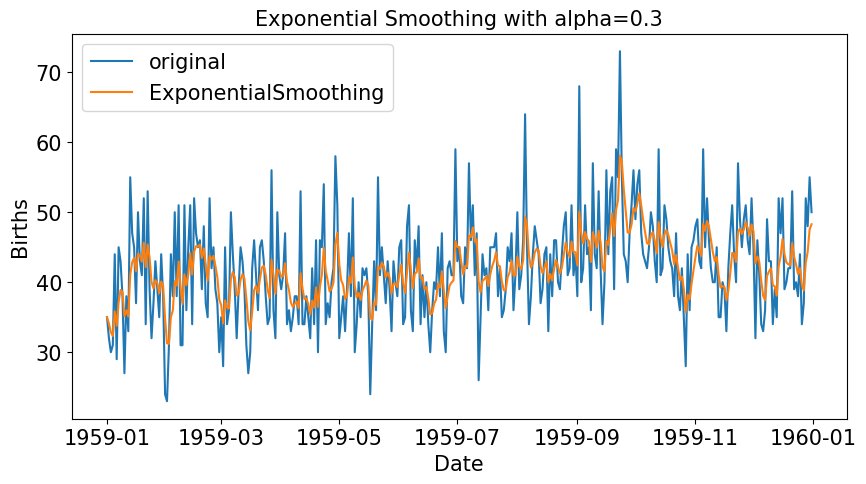
\includegraphics{../images/02/Exponential_Smoothing.png}

\hypertarget{double-exponential-smoothing-holts-method}{%
\subsection{Double Exponential Smoothing (Holt's Method)}\label{double-exponential-smoothing-holts-method}}

\hypertarget{triple-exponential-smoothing-holt-winters-method}{%
\subsection{Triple Exponential Smoothing (Holt-Winters' Method)}\label{triple-exponential-smoothing-holt-winters-method}}

\hypertarget{autoregressive-model}{%
\chapter{Autoregressive Model}\label{autoregressive-model}}

\hypertarget{muxf4-huxecnh-tux1ef1-hux1ed3i-quy-luxe0-guxec}{%
\section{Mô hình tự hồi quy là gì}\label{muxf4-huxecnh-tux1ef1-hux1ed3i-quy-luxe0-guxec}}

Mô hình tự hồi quy là mô hình ước lượng giá trị tương lai của timeseries dựa vào các giá trị trong quá khứ cửa chính timeseries đó.

Công thức tự hồi quy được biểu diễn như sau

\[
y_t = c + \theta_1 y_{t-1} + \theta_2 y_{t-2} + \theta_3 y_{t-3} + .... + \theta_p y_{t-p} + \epsilon_t
\]

Trong đó: \(\epsilon_t\) là nhiễu trắng. Có thể nói mô hình này là mô hình hồi quy đa biến với các biến là các giá trị lag tại thời điểm từ \(1\) đến \(p\). Chúng ta kí hiệu mô hình này là \(AR(p)\)

Để sử dụng AR model, ta dùng class \texttt{AutoReg} của thư viện \texttt{statsmodels}, chúng ta dùng \texttt{root\_mean\_squared\_error} để đánh giá mô hình. Mô hình sẽ được huấn luyện và dự đoán cho 7 ngày tiếp theo

\begin{Shaded}
\begin{Highlighting}[]

\ImportTok{from}\NormalTok{ statsmodels.tsa.ar\_model }\ImportTok{import}\NormalTok{ AutoReg}
\ImportTok{import}\NormalTok{ pandas }\ImportTok{as}\NormalTok{ pd }
\ImportTok{import}\NormalTok{ numpy }\ImportTok{as}\NormalTok{ np}

\CommentTok{\# Đọc dữ liệu}
\NormalTok{df }\OperatorTok{=}\NormalTok{ pd.read\_csv(}\StringTok{\textquotesingle{}../data/us{-}retail{-}sales.csv\textquotesingle{}}\NormalTok{)}

\CommentTok{\# Chia dữ liệu thành train test}
\NormalTok{Y }\OperatorTok{=}\NormalTok{ df.Clothing.values}
\NormalTok{train, test }\OperatorTok{=}\NormalTok{ Y[:}\BuiltInTok{len}\NormalTok{(Y)}\OperatorTok{{-}}\DecValTok{7}\NormalTok{], Y[}\BuiltInTok{len}\NormalTok{(Y)}\OperatorTok{{-}}\DecValTok{7}\NormalTok{:]}

\CommentTok{\# Huấn luyện mô hình với p=29}
\NormalTok{model }\OperatorTok{=}\NormalTok{ AutoReg(train, lags}\OperatorTok{=}\DecValTok{29}\NormalTok{)}
\NormalTok{model\_fit }\OperatorTok{=}\NormalTok{ model.fit()}

\CommentTok{\# Dự đoán kết quả mô hình}
\NormalTok{Y\_hat }\OperatorTok{=}\NormalTok{ model\_fit.predict(start}\OperatorTok{=}\BuiltInTok{len}\NormalTok{(train), end}\OperatorTok{=}\BuiltInTok{len}\NormalTok{(train)}\OperatorTok{+}\BuiltInTok{len}\NormalTok{(test)}\OperatorTok{{-}}\DecValTok{1}\NormalTok{, dynamic}\OperatorTok{=}\VariableTok{False}\NormalTok{)}
\ControlFlowTok{for}\NormalTok{ y\_hat, y\_true }\KeywordTok{in} \BuiltInTok{zip}\NormalTok{(Y\_hat, test):}
    \BuiltInTok{print}\NormalTok{(}\SpecialStringTok{f\textquotesingle{}Predicted=}\SpecialCharTok{\{}\NormalTok{y\_hat}\SpecialCharTok{\}}\SpecialStringTok{ }\CharTok{\textbackslash{}t}\SpecialStringTok{Expected=}\SpecialCharTok{\{}\NormalTok{y\_true}\SpecialCharTok{\}}\SpecialStringTok{\textquotesingle{}}\NormalTok{)}
\end{Highlighting}
\end{Shaded}

\begin{Shaded}
\begin{Highlighting}[]
\NormalTok{Predicted}\OperatorTok{=}\FloatTok{21279.50586647284}\NormalTok{     Expected}\OperatorTok{=}\DecValTok{21116}
\NormalTok{Predicted}\OperatorTok{=}\FloatTok{22101.240803540295}\NormalTok{    Expected}\OperatorTok{=}\DecValTok{21742}
\NormalTok{Predicted}\OperatorTok{=}\FloatTok{23214.72663871385}\NormalTok{     Expected}\OperatorTok{=}\DecValTok{23829}
\NormalTok{Predicted}\OperatorTok{=}\FloatTok{19752.699859625853}\NormalTok{    Expected}\OperatorTok{=}\DecValTok{19567}
\NormalTok{Predicted}\OperatorTok{=}\FloatTok{21334.77904024157}\NormalTok{     Expected}\OperatorTok{=}\DecValTok{21400}
\NormalTok{Predicted}\OperatorTok{=}\FloatTok{25209.963983161964}\NormalTok{    Expected}\OperatorTok{=}\DecValTok{25170}
\NormalTok{Predicted}\OperatorTok{=}\FloatTok{34357.54441580368}\NormalTok{     Expected}\OperatorTok{=}\DecValTok{35157}
\end{Highlighting}
\end{Shaded}

Để xem các params của mô hình ta gọi \texttt{model\_fit.params}. Trong đó giá trị đầu tiên là hằng số \(c\), các giá trị tiếp theo tương ứng là các \(\theta\) tại các lag

\begin{Shaded}
\begin{Highlighting}[]
\NormalTok{model\_fit.params}
\end{Highlighting}
\end{Shaded}

\begin{verbatim}
array([ 2.28853925e+02,  1.79171595e-01,  2.54201532e-01,  3.05500421e-01,
       -3.11981291e-02,  6.65420755e-02,  1.10686710e-01, -3.19428627e-02,
        4.96965486e-02,  8.89945569e-02, -1.20435797e-01, -3.84651164e-02,
        8.06193600e-01, -1.26996681e-01, -1.27501050e-01, -2.69789259e-01,
       -1.01531188e-01, -4.45741520e-02, -1.10645162e-01,  3.58745006e-02,
       -4.99340277e-02, -9.73275266e-02,  1.14918312e-01,  4.15776199e-02,
        2.03791299e-01, -6.05281674e-02, -1.38168187e-01, -3.51125341e-02,
        1.36761315e-01, -1.65243492e-02])
\end{verbatim}

Để đánh giá kết quả mô hình, chúng ta dùng thư viện \texttt{sklearn.metrics}

\begin{Shaded}
\begin{Highlighting}[]
\ImportTok{from}\NormalTok{ sklearn.metrics }\ImportTok{import}\NormalTok{ mean\_squared\_error}
\BuiltInTok{print}\NormalTok{(}\StringTok{\textquotesingle{}RMSE:\textquotesingle{}}\NormalTok{, np.sqrt(mean\_squared\_error(test, Y\_hat)))}
\end{Highlighting}
\end{Shaded}

\begin{verbatim}
416.20469692462274
\end{verbatim}

Dưới đây là biểu đồ thể hiện giá trị Dự đoán và giá trị thực tế trong 7 ngày

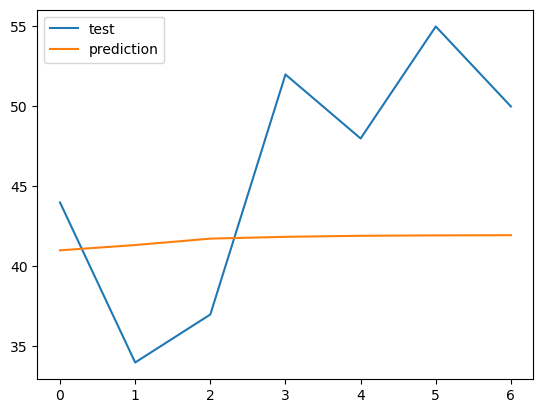
\includegraphics{../images/03/autoregressive.png}

\printindex

\end{document}
